\begin{center}
\Huge
Cirkler og linjer
\end{center}

\section*{Skæring mellem cirkel og linje}
\stepcounter{section}
Vi skal afgøre, hvordan vi bestemmer skæringspunkter mellem cirkler og linjer. Vi ser derfor på et eksempel.
\begin{exa}
	Lad os betragte en cirkel $C$ med centrum i $(4,2)$ og radius 8. Denne 
	cirkel har ligningen 
	\begin{align*}
		(x-4)^2 + (y-2)^2 = 64.
	\end{align*}
	Lad os desuden betragte en linje $l$ med ligningen
	\begin{align*}
		l: \ 2(x-1) -2(y-3) = 0. 
	\end{align*}
	Disse kan ses på Fig. \ref{fig:cirkellinje}.
	\begin{figure}[H]
		\centering
		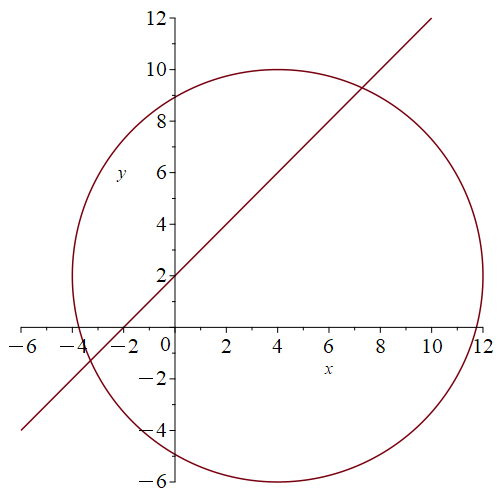
\includegraphics[width=0.6\textwidth]{Billeder/cirkellinje.png}
		\caption{Cirklen $C$ og linjen $l$.}
		\label{fig:cirkellinje}
	\end{figure}
	Vi kan bestemme skæringspunkterne mellem disse i Maple. De bestemmes til at være $(-3.3, -1.3)$ og $(7.3,9.3)$. 
\end{exa}

\section*{Tangent til cirkel}
\stepcounter{section}

En tangent til en cirkel er en ret linje, der følger langs en cirkel og som rører cirklen i netop ét punkt. Kender vi centrum til en cirkel samt et punkt, hvor vi ønsker en tangent, så kan vi bestemme en tangent til cirklen i lige netop det punkt. Lad os betragte et eksempel. Idéen kan ses på Fig. \ref{fig:cirkeltangent}.
\begin{figure}[H]
	\centering
	\resizebox{0.5\textwidth}{0.5\textwidth}
	{
	\begin{tikzpicture}
		\begin{axis}[axis lines = middle, 
		ticks = none,
		xmin = -2, xmax = 8,
		ymin = -2, ymax = 8]
			\draw[thick, color = blue!40] (axis cs: 2,3) circle[radius = 4];
			\draw[-{Stealth[scale = 1.3]}] (axis cs: 4.59,6.05) to (axis cs:2,3);
			\addplot[color = red!40, thick, domain = -2:8] {-0.849*x+9.964};
			\filldraw[color = purple] (axis cs: 4.59,6.05) circle[radius =2pt];
			\filldraw[color = purple] (axis cs: 2,3) circle[radius =2pt];
		\end{axis}
	\end{tikzpicture}
	}
\end{figure}
\begin{exa}
	En cirkel med centrum i $C(-2,3)$ og radius $4$ er givet. Punktet $P(1.94, 3.68)$ ligger på cirklen. Vi skal bestemme ligningen for tangenten til cirklen, der går gennem
	dette punkt. En normalvektor til tangenten er givet ved
	\begin{align*}
		\vv{CP} = 
		\begin{pmatrix}
			-3.94 \\ -0.68
		\end{pmatrix}.
	\end{align*}
	Desuden går tangentlinjen selvfølgelig igennem punktet $P$. Derfor kan vi indsætte dette i cirklens ligning
	\begin{align*}
		a(x-x_0) + b(y-y_0)=0,
	\end{align*}
	og vi får
	\begin{align*}
		-3.94(x-1.94) -0.68(y-3.68) = 0
	\end{align*}
	som tangentens ligning. 
\end{exa}

\section*{Opgave 1}
\begin{enumerate}[label=\roman*)]
	\item En cirkel har ligningen $(x+2)^2+(y-2)^2 = 4,$ og en linje har ligningen $y=-x$. Bestem skæringspunkterne mellem cirklen og ligningen.
	\item En cirkel har ligningen $(x)^2+(y-3)^2 = 16,$ og en linje har ligningen $1(x-2)-2(y-1)=0$. Bestem skæringspunkterne mellem cirklen og ligningen.
	\item En cirkel har ligningen $x^2+2x+y^2+4y = 4,$ og en linje har ligningen $4(x+3)+3(y+3)=0$. Bestem skæringspunkterne mellem cirklen og ligningen.
	\item En cirkel har ligningen $x^2+y^2=1,$ og en linje har ligningen $y=1$. Bestem skæringspunkterne mellem cirklen og ligningen.
\end{enumerate}

\section*{Opgave 2}
\begin{enumerate}[label=\roman*)]
	\item En cirkel har centrum i $(-5,4)$ og radius $3$, og en linje har ligningen $y = 2x+10$. Bestem skæringspunkterne mellem cirklen og ligningen
	\item En cirkel har ligningen $(x+2)^2+(y-7)^2 = 100$ og en linje har normalvektoren 
	\begin{align*}
		\vv{n} =
		\begin{pmatrix}
			2 \\ 1
		\end{pmatrix}
	\end{align*}
	og går gennem punktet $(-5,4)$. Bestem skæringspunkterne mellem cirklen og linjen. 
	\item En cirkel har centrum i $(1,1)$ og radius $2$, og en linje har normalvektor 
	\begin{align*}
		\vv{n} =
		\begin{pmatrix}
			-4 \\ -7			
		\end{pmatrix}
	\end{align*}
	og går gennem punktet $(1,3)$. Bestem skæringspunkterne mellem cirklen og linjen
\end{enumerate}

\section*{Opgave 3}
\begin{enumerate}[label=\roman*)]
	\item	En cirkel er givet ved ligningen $(x-2)^2 + (y-3)^2 = 4$ og punktet $(3.14,4.64)$
	ligger på cirklen. Bestem ligningen for tangenten til cirklen gennem dette punkt.
	\item	En cirkel er givet ved ligningen $(x+1)^2 + (y+2)^2 = 25$ og punktet
	 $(-5.75,-3.56)$
	ligger på cirklen. Bestem ligningen for tangenten til cirklen gennem dette punkt.	
	\item	En cirkel har centrum i $(-3,6)$ og punktet
	 $(-10,9)$
	ligger på cirklen. Bestem ligningen for tangenten til cirklen gennem dette punkt.	
	\item	En cirkel er givet ved ligningen $x^2-4x+y^2-8y=16$ og punktet
	 $(4.70,-1.36)$
	ligger på cirklen. Bestem ligningen for tangenten til cirklen gennem dette punkt.	
\end{enumerate}

\section*{Opgave 4}
\begin{enumerate}[label=\roman*)]
	\item En cirkel har centrum i $(2,y_0)$ og radius $5$. Bestem tallet $y_0$, så linjen $2(x-2) + 4(y-1) = 0$ 
	er tangent til cirklen.
	\item En cirkel har centrum i $(5,4)$ og radius $7$. Bestem tallet $k$, så linjen $-6(x-k)-9(y+3) = 0$ er 
	tangent til cirklen.
	\item En cirken har centrum i $(7,1)$. Bestem radius for cirklen, så linjen $-2(x+3)-5(y-11)$ er tangent
	til cirklen. 
\end{enumerate}
